\chapter{The Physics of Accretion}

\label{sec:PhysAcc}

\epigraph{\textit{A black hole consumes matter, sucks it in, and crushes it beyond existence. When I first heard that, I thought that's evil in its most pure.}}{Alice Morgan -- \textit{Luther}}

\vspace{1cm}

\par\noindent The extreme environments in accreting systems lead to a variety of somewhat unintuitive physical effects and phenomena.  In this chapter, I explain a number of these effects, and delve into the history of physical and mathematical models which have been proposed to explain the effects seen in X-ray binaries.

\section{The Eddington Limit}

\par Consider an element of gas at distance $r$ from a compact object, with mass $m$.  This element of gas is acted on by a inwards-pointing gravitational force given by:
\begin{equation}
F_G=\frac{GMm}{r^2}
\end{equation}
Where $M$ is the mass of the compact object.
\par The X-ray Binary is of course bright in electromagnetic radiation, emitting a luminosity $L$.  If we assume that this luminosity is emitted isotropically from the compact object, then the electromagnetic flux at distance $r$ is given by:
\begin{equation}
\phi(r)=\frac{L}{4\pi r^2}
\end{equation}
Electromagnetic radiation exerts a pressure on material corresponding to $\phi/c$.  As such, the radiation from the X-ray binary exerts an outwards force on our gas element corresponding to:
\begin{equation}
F_L=\frac{\kappa m\phi(r)}{c}=\frac{L\kappa m}{4\pi r^2c}
\end{equation}
Where $\kappa$ is the opacity of the cloud, or its surface area per unit mass.
\par If $F_G$ and $F_L$ are equal, then no net force is exerted on our cloud of matter and it will not accrete onto the compact object.  This happens when:
\begin{eqnarray}
F_G&=&F_L\\ \nonumber \\
\frac{GMm}{r^2}&=&\frac{L\kappa m}{4\pi r^2c} \\ \nonumber \\
L&=&\frac{GMm}{r^2}\frac{4\pi r^2c}{\kappa m} \\ \nonumber \\
L&=&\frac{4\pi GMc}{\kappa}
\end{eqnarray}
This luminosity, denoted as $L_E$, is the Eddington luminosity of the source; the theoretical maximum luminosity an object can be and still have accretion take place.  It only depends on the mass of the compact object $M$ and the opacity of the accreting material $\kappa$, which in turn depends on the chemical make-up of the accretion disk.  As accretion disks tend to be dominated by ionised hydrogen, $\kappa$ is usually assumed to be $\sigma_T/m_p$, where $\sigma_T$ is the Thomson scattering cross section of an electron and $m_p$ is the mass of a proton.  This assumption yields the final formula which only depends on the mass of the compact object:
\begin{equation}
L_E=\frac{4\pi GMm_pc}{\sigma_T}
\end{equation}
The luminosity due to matter falling into a black hole can be expressed as:
\begin{equation}
L=\eta\dot{M}c^2
\end{equation}
Where $\dot{M}$ is the accretion rate and $\eta$ is the efficiency at which the gravitational potential energy of infalling matter is converted to outgoing radiation.  As such, $L_E$ also corresponds to a theoretical maximum accretion rate.
\par However, a number of X-ray binaries have been seen to shine at luminosities far above this limit; in one of the most extreme cases, the confirmed neutron star XRB M82 X-1 has a luminosity of $\sim100L_E$ \citep{Bachetti_M82X1}.  This super-Eddington accretion is possible due to the fact that a number of assumptions made when calculating the Eddington limit do not apply to physical XRBs.  In particular, the calculation performed above assumes that both accretion on to the compact object, as well as electromagnetic emission from it, are isotropic.  An object may exceed the Eddington Limit if it is accreting anisotropically, which is the case for XRBs as these systems accrete from near-planar disks.  A system may appear to further exceed the Eddington limit if its emission is beamed; an XRB beaming its radiation in the direction of the Earth would lead us to infer an artificially high value of $L$, and thus overestimate its luminosity with respect to the Eddington Limit.
\par Despite these setbacks, the Eddington Luminosity is a useful tool to compare XRBs with different compact object masses.  By expressing the luminosity of an object as a fraction of its Eddington Limit, often referred to as its Eddington fraction, objects can be rescaled in such a way that we can compare how dominant photon pressure must be in each accretion disk.

\section{The Propeller Effect}

\label{sec:prop}

\par Another limit on accretion rate arises when one considers the effect of a strong neutron star magnetic field.  To understand this effect, we must first define two characteristic radii of such a system.
\par First, assume that the magnetic field of the neutron star can be approximated as a set of rigid field lines which are anchored to points on the neutron star surface.  The magnetic field can then be thought of as a `cage' which rotates with the neutron star at its centre.  The straight-line speed of a point on this rotating cage is given by:
\begin{equation}
v_\nu(r)=2\pi r\nu
\end{equation}
Where $r$ is the distance from the neutron star centre and $\nu$ is the rotation frequency of the neutron star.  This can be compared with the Keplerian speed, or the speed of a particle in a Keplerian orbit around the compact object.  This is given by:
\begin{equation}
v_K(r)=\sqrt{\frac{GM}{r}}
\end{equation}
Where $M$ is the mass of the neutron star.  By setting these equal, we can find the radius at which the magnetic field is rotating at the same speed as a particle in a Keplerian orbit:
\begin{eqnarray}
v_\nu(r)&=&v_K(r)\\ \nonumber \\
2\pi r\nu&=&\sqrt{\frac{GM}{r}}\\ \nonumber \\
r^3&=&\frac{GM}{4\pi^2\nu^2}\\ \nonumber \\
r&=&\sqrt[3]{\frac{GM}{4\pi^2\nu^2}}
\end{eqnarray}
This radius is denoted as $r_c$, the co-rotation radius.  Inside of this radius, a particle in an equatorial Keplerian orbit has a greater velocity than the magnetic field lines; outside this radius, the magnetic field lines are moving faster.  To understand the significance of this radius, we must define another characteristic radius of the system.
\par In a neutron star accretion disk, there are three significant sources of pressure: gas (or ram) pressure $P_g$, photon pressure $P_\gamma$ and magnetic pressure $P_\mu$.  Whichever pressure is dominant in a given location will govern the physics of matter in that region.
\par Photon pressure falls off sharply outwards from the inner disk, so it can be assumed to be negligible in the region of the disk considered here.  We can then calculate where in the disk each of the remaining two pressures dominates.
\par Assuming that the field of the neutron star is a magnetic dipole, the magnetic pressure at a point a distance $r$ above its equator can be given as:
\begin{eqnarray}
P_\mu&=&\frac{B^2}{2\mu_0}\\ \nonumber \\
B(r)&=&B_0\left(\frac{R_{NS}}{r}\right)^3\label{eq:NS}\\ \nonumber \\
\therefore\quad P_\mu&=&\frac{B_0^2}{2\mu_0}\left(\frac{R_{NS}}{r}\right)^6
\end{eqnarray}
Where $\mu_0$ is the vacuum permeability, $B_0$ is the equatorial magnetic field strength at the neutron star surface, $R_{NS}$ is the radius of the neutron star and Equation \ref{eq:NS} is the equation for the magnetic field strength above the equator of a dipole.
\par The functional form of the ram pressure depends on the assumed accretion geometry of the system.  As when calculating the Eddington Limit, one can assume the simplest possible case of spherically accreting free-falling matter.  The ram pressure is then given by:
\begin{equation}
P_g=\frac{\dot{M}}{4\pi r^2}\sqrt{\frac{2GM}{r}}
\end{equation}
When $P_\mu>P_g$, accreting material is dominated by magnetic pressure in such a way that material is `frozen' onto magnetic field lines \citep{Alfven_Waves}; this results in material flowing onto the neutron star surface along magnetic field lines onto the poles, as described in section \ref{sec:NSintro}.  It is possible to express the region of the accretion disk within which matter is magnetically dominated:
\begin{eqnarray}
P_g&<&P_\mu\\ \nonumber \\
\frac{\dot{M}}{4\pi r^2}\sqrt{\frac{2GM}{r}}&<&\frac{B_0^2}{2\mu_0}\left(\frac{R_{NS}}{r}\right)^6\\ \nonumber \\
\frac{GM\dot{M}^2}{8\pi^2 r^5}&<&\frac{B_0^4}{4\mu_0^2}\left(\frac{R_{NS}}{r}\right)^{12}\\ \nonumber \\
r^7&<&\frac{2\pi^2}{G\mu_0^2}\frac{B_0^4R_{NS}^{12}}{M\dot{M}^2}\\ \nonumber \\
r&<&\sqrt[7]{\frac{2\pi^2}{G\mu_0^2}\frac{B_0^4R_{NS}^{12}}{M\dot{M}^2}}
\end{eqnarray}
The critical radius, the magnetospheric or Alfv\'en radius, is denoted as $r_\mu$.
\par Now it is possible to consider what happens to matter approaching $r_\mu$ in two different physical regimes.  First of all, consider a system in which the corotation radius $r_c>r_\mu$.  In this case, magnetic field lines at $r_\mu$ are moving slower than the Keplerian speed.  An element of matter approaching this radius from a Keplerian orbit will experience a torque slowing it down as it freezes onto the field lines.  By Kepler's laws of planetary motion, this necessarily decreases the altitude of this element of matter.  This pulls the element further into the magnetically-dominated regime and allows it to accrete freely along the field line onto the neutron star.
\par Now consider what happens when $r_c<r_\mu$.  In this case, field lines at $r_\mu$ are moving faster than the Keplerian speed.  An element of matter approaching $r_\mu$ will therefore experience a torque speeding it up as it becomes frozen onto magnetic field lines.  This will increase its altitude, driving it back away from $r_\mu$.  In this case, the magnetospheric radius acts as a barrier to infalling matter, repelling any gas that approaches it and stopping accretion onto the neutron star surface.  This set of circumstances is known as the `propeller regime', due to the rapidly rotating field lines acting like a `propeller' which blow the inner part of the disk away.
\par As the propeller regime is expected to occur for $r_c<r_\mu$, it is possible to work out what kind of system this should be observed in:
\begin{eqnarray}
r_c&<&r_\mu\\ \nonumber \\
\left(\frac{GM}{4\pi^2\nu^2}\right)^{1/3}&<&\left(\frac{2\pi^2}{G\mu_0^2}\frac{B_0^4R_{NS}^{12}}{M\dot{M}^2}\right)^{1/7}\\ \nonumber \\
M^{10/21}\dot{M}^{2/7}&<&k\nu^{2/3}B_0^{4/7}R_{NS}^{12/7}
\end{eqnarray}
Where $k$ is a constant.  Assuming that the radius and mass of neutron stars does not vary much, this inequality tells us that the propeller regime is more likely to be observed in neutron star XRBs with a high spin frequency and a high magnetic field.  It also tells us that the propeller effect places a \textit{lower} limit on accretion in such systems: accretion is not possible unless infalling matter can apply enough ram pressure to push the magnetospheric radius inside the corotation radius.
\par There are numerous problems with this relatively simplistic view of accretion in a highly magnetic regime.  Much as in the calculation of the Eddington Limit, it is not clear that all the assumptions are physical.  This calculation again depends on an unphysical spherical accretion geometry, and makes the assumption that the magnetic field lines can in no way be warped by the movement of ionised matter on them.  Additionally \citet{White_MRad} show that the magnetospheric radius calculated for neutron stars may fall close enough to the inner edge of the disk that photon pressure cannot be safely ignored.  In this scenario, calculating the magnetospheric radius becomes much less straightforward.  Despite these difficulty, an effect observationally similar to the propeller effect is observed in a number of astrophysical neutron star XRBs (e.g. \citealp{Fabian_Propex,Furst_Propex}) and other systems (e.g. \citep{Campana_PropBorder}), and as such it is likely that effect similar to this can explain what we see in nature.

\section{The Shakura-Sunyaev Disk Model}

\par To understand how the very non-spherical nature of accretion disks affects their physics, it is important to construct models.  Much of our understanding of the physics of astrophysical accretion disks stems from a model proposed by Nikolai Shakura and Rashid Sunyaev in 1973 \citep{Shakura_Disk}.  This model specifically considered the effects of accretion onto a black hole.  By showing that this would result in a system which would be bright in the X-ray, and describing how such a system would appear, this model proved pivotal in the scientific community's acceptance of the earliest XRB identifications (e.g.\citealp{Bolton_CygX1}).
\par \citeauthor{Shakura_Disk} model the accretion disk as a structure held up by centrifugal forces, generated by the large amount of angular momentum possessed by infalling matter due to the orbit of the binary system.  Frictional forces cause this angular momentum to be transferred outwards, heating up the disk and allowing matter to fall in towards the black hole.  The efficiency with which this angular momentum is transferred, parameterised as $\alpha$, can then be thought of as a measure of the viscosity of the disk.
\par \citeauthor{Shakura_Disk} base their calculations on Newtonian mechanics; as such they ignore the region of the disk inwards of the ISCO at $r=3r_g$, where relativistic effects become important.  They also assume that the disk in a steady state, that it is geometrically thin (such that height of the disk $H\ll r$ everywhere) and that it is cylindrically symmetric.  The last two assumptions allow us to write down formulae for the surface density $\Sigma$, radial velocity $u_r$ and accretion rate $\dot{M}$ of the disk as a functions of radius $r$:
\begin{eqnarray}
\Sigma(r)&=&\int_{-H}^H\rho(r,z) dz\label{eq:base1}\\\nonumber \\
u_r(r)&=&\frac{1}{\Sigma(r)}\int_{-H}^H\rho(r,z)v_r(r,z)dz\label{eq:base2}\\\nonumber \\
\dot{M}(r)&=&-2\pi r\Sigma(r) u_r(r)\label{eq:base3}
\end{eqnarray}
Where $\rho(r,z)$ is the density at a radius $r$ and height $z$, and $v_r$ is the radial velocity of the gas at this point.
\par Now consider the Euler equations of hydrodynamics:
\begin{eqnarray}
\frac{\partial\rho}{dt}+\dv(\rho\bm{v})&=&0\label{eq:consmass}\\\nonumber \\
\rho\left(\frac{\partial\bm{v}}{dt}+(\bm{v}\cdot\dv) \bm{v}\right)&=&-\dv p\label{eq:fma}
\end{eqnarray}
Where Equation \ref{eq:consmass} is the conservation of mass and Equation \ref{eq:fma} is a differential form of Newton's second law of motion.  These equations can be cast in cylindrical co-ordinates to give 4 equations: the recast continuity equation and one motion equation for each of the radial ($r$), vertical ($z$) and azimuthal ($\theta$) directions:
\begin{eqnarray}
\frac{\partial\rho}{\partial t}+\frac{1}{r}\frac{\partial(r\rho v_r)}{\partial r}+\frac{1}{r}\frac{\partial v_\theta}{\partial\theta}+\frac{\partial v_z}{\partial z}&=&0\label{eq:ssc}\\\nonumber\\
\rho\left(\frac{\partial v_r}{\partial t}+v_r\frac{\partial v_r}{\partial r}+\frac{v_\theta}{r}\frac{\partial v_r}{\partial\theta}+v_z\frac{\partial v_r}{\partial z}-\frac{v_\theta^2}{r}\right)&=&\frac{-\partial p}{\partial r}\label{eq:ssr}\\\nonumber\\
\rho\left(\frac{\partial v_\theta}{\partial t}+v_r\frac{\partial v_\theta}{\partial r}+\frac{v_\theta}{r}\frac{\partial v_\theta}{\partial\theta}+v_z\frac{\partial v_\theta}{\partial z}+\frac{v_rv_\theta}{r}\right)&=&\frac{-\partial p}{\partial\theta}\\\nonumber\\
\rho\left(\frac{\partial v_z}{\partial t}+v_r\frac{\partial v_z}{\partial r}+\frac{v_\theta}{r}\frac{\partial v_z}{\partial\theta}+v_z\frac{\partial v_z}{\partial z}\right)&=&\frac{-\partial p}{\partial z}\label{eq:ssz}
\end{eqnarray}
By the assumptions that the disk is in a steady state and cylindrically symmetric, we can set all $\frac{\partial}{\partial\theta}$ and $\frac{\partial}{\partial t}$ terms to zero, simplifying equations \ref{eq:ssr} to \ref{eq:ssz}:
\begin{eqnarray}
\rho\left(v_r\frac{\partial v_r}{\partial r}+v_z\frac{\partial v_r}{\partial z}-\frac{v_\theta^2}{r}\right)&=&\frac{-\partial p}{\partial r}\label{eq:ssrs}\\\nonumber\\
\rho\left(v_r\frac{\partial v_\theta}{\partial r}+v_z\frac{\partial v_\theta}{\partial z}+\frac{v_rv_\theta}{r}\right)&=&0\label{eq:ssts}\\\nonumber\\
\rho\left(v_r\frac{\partial v_z}{\partial r}+v_z\frac{\partial v_z}{\partial z}\right)&=&\frac{-\partial p}{\partial z}\label{eq:sszs}
\end{eqnarray}
We can average the density term on left-hand side of Equation \ref{eq:ssc} in the $z$-direction, and substitute in the results from Equations \ref{eq:base1} to \ref{eq:base3} to find:
\begin{eqnarray}
\frac{1}{r}\frac{d}{dr}\left(r\int_{-H}^H\rho v_rdz\right)&=&0\\\nonumber\\
\frac{1}{r}\frac{d(r\Sigma u_r)}{dr}&=&0\\\nonumber\\
\frac{-1}{2\pi r}\frac{d\dot{M}}{dr}&=&0
\end{eqnarray}
Therefore the rate of inwards matter flow $\dot{M}$ is constant at all $r$.
\par Using the fact that the angular velocity $\omega$ of an element in the gas can be written as $\omega=v_\theta/r$, we can re-write Equation \ref{eq:ssrs} as:
\begin{equation}
\rho\left(v_r\frac{\partial v_r}{\partial r}-\omega^2r\right)=-\frac{\partial p}{\partial r}-\rho v_z\frac{GM}{r^2}
\end{equation}
Where the term $\frac{GM}{r^2}$ has been introduced to account for the fact that the gradient of the gravitational field in the $r$ direction is non-zero.  This leads to:
%We can rewrite $v_z\frac{\partial v_r}{\partial z}$ as $\frac{\partial v_r}{\partial z}\frac{\partial z}{\partial t}$, which is equal to the inwards acceleration of a gas element moving in the $z$-direction.  As the disk is assumed to be in a cylindrically symmetric gravitational potential, this acceleration can be given by $\dot{v}_r=\frac{GM}{r^2}$.
\begin{equation}
\rho\left(v_r\frac{\partial v_r}{\partial r}-\omega^2r\right)=-\frac{\partial p}{\partial r}-\rho\omega_k^2r
\end{equation}
Assuming that is thin and angular momentum is only transferred slowly, i.e. $v_r\frac{\partial v_r}{\partial r}\ll\omega$, this leads to:
\begin{equation}
\omega\approx\omega_k
\end{equation}
Showing that gas elements in the disk orbit at Keplerian speeds.
\par Using similar logic, Equation \ref{eq:sszs} becomes:
\begin{equation}
\rho\omega_k^2 z=\frac{-\partial p}{\partial z}\label{eq:idgas}
\end{equation}
The ideal gas law $p=\rho RT$\footnote{$R$ is the specific gas constant, equal to the Boltzmann Constant $k_B$ divided by the mean molar mass of the gas.} can then be used to rewrite equation \ref{eq:idgas}:
\begin{equation}
\frac{p}{RT}\omega_k^2 z=\frac{-\partial p}{\partial z}\label{eq:idgas2}
\end{equation}
If we assume that the disk is chemically homogeneous and isothermal in the $z$-direction, then neither $R$ nor $T$ depend on $z$.  Equation \ref{eq:idgas2} then admits the solution:
\begin{equation}
\rho=\rho_0(r)e^{\left(\frac{-z^2\omega_k^2}{2RT}\right)}=\rho_0(r)e^{\frac{-z^2}{2H^2}}
\end{equation}
Where $\rho_0$ is the density at radius $r$ when $z=0$.  As such, the density of the disk has a Gaussian profile in the $z$-direction, with a scale-width $H_s$ given by:
\begin{equation}
H_s=\frac{\sqrt{RT}}{\omega_k}
\end{equation}
This shows that the scale height of the disk is finite for all $r$.  As the integral between $-\infty$ and $+\infty$ of a Gaussian with a finite scale-width is finite, the disk contains a finite amount of matter.
\par Finally, \citeauthor{Shakura_Disk} looked at the solutions to Equation \ref{eq:ssts}.  As every term in this equation depends on either $v_\theta$ or a derivative thereof, this equation admits the solutions $\rho=0$ or $v_\theta=0$.  Both of these solutions imply accretion rates of zero, as any matter in the disk must have a non-zero density and angular momentum.  In order to resolve this problem, \citet{Shakura_Disk} add the divergence of the viscous stress tensor \citep{Landau_Tensor} to the right-hand side of Equation \ref{eq:ssts} to represent the effects of viscosity within the disk.  By doing this, they find the following two results:
\begin{eqnarray}
\dot{M}&=&\frac{4\pi H\eta_b r}{\omega}\frac{\partial\omega}{\partial r}\label{eq:diffrot}\\\nonumber\\
\dot{M}&=&6\pi\eta_b H\label{eq:viscos}
\end{eqnarray}
Equation \ref{eq:diffrot} confirms that the disk is a differential rotator, while Equation \ref{eq:viscos} confirms that accretion can only take place when $\eta_b$ (the bulk viscocity) is non-zero.
\par \citet{Shakura_Disk} found that molecular viscosity alone cannot be high enough to result in the high values of $\dot{M}$ inferred for observed XRBs.  Instead, the authors assume that turbulence is present in the disk.  Using formulae pertaining to turbulent hydrodynamics, and by ignoring supersonic perturbations, they find an upper bound on bulk viscosity $\eta$:
\begin{equation}
\eta_b\leq\frac{2}{3}\rho_0H\sqrt{RT}
\end{equation}
As such, they define their dimensionless viscosity parameter $\alpha$ as:
\begin{equation}
\alpha\equiv\frac{3\eta_b}{2\rho_0H\sqrt{RT}}\quad\quad\quad\alpha\leq1
\end{equation}

\subsection{The source of Turbulence}

\par \citet{Shakura_Disk} do not answer the question of what physical process causes the turbulence required to stabilise accretion disks.  \citet{Balbus_MRI} were among the first to propose the Magnetorotational Instability \citep[MRI,][]{Velikhov_MRI,Chandrasekhar_MRI} as the source of this turbulence.  MRI is a process which occurs in an ionised and differentially rotating disk.  Fluctuations in the material in the disk generate internal magnetic fields.  The field lines associated with these fields, in general, extend a finite distance in the radial direction, thus connecting gas elements at different radii.  As gas elements in a Shakura-Sunyaev accretion disk orbit the compact object at Keplerian speeds, elements of gas at different radii move at different orbital speeds.  As such, these internal magnetic field lines become stretched as gas orbits the compact object.  This field line stretching imparts a torque on the gas elements, causing the outer, slower element to speed up and the inner, faster element to slow down.  As such, the net result of this process is an outwards transfer of angular momentum.
\par \citet{Balbus_MRI} found that the angular momentum transfer due to MRI was more significant than that due to friction, hydrodynamic turbulence or other sources in an accretion disk.  They suggest therefore that MRI is the main component of outwards angular momentum transfer, and thus of $\alpha$, in astrophysical accretion disks.

\subsection{Disk Instabilities}

\label{sec:diskinstab}

\par A number of effects can cause an accretion disk, or portions of it, to become unstable.  Some of these instabilities can set up limit cycles of behaviour in the disk, resulting in quasi-periodic fluctuations in the object's intensity or colour as seen from Earth.  I describe a number of these instabilities here.
\par One of the first such instabilities to be discovered was first described by \citealp{Lightman_Instability}.  Using the assumptions present in the thin disk models of \citet{Shakura_Disk} and \citet{Novikov_Torque}, \citeauthor{Lightman_Instability} show that an annulus within a thin, radiatively dominated disk has an effective negative radial diffusion coefficient.  As such, any initially smooth disk under these conditions tends to separate into dense annuli.  As such any sufficiently thin disk, with $\alpha$ consistent with the prescription of \citet{Shakura_Disk} is unstable.
\par \citet{Shakura_Instab} described another instability which takes place in the radiation pressure-dominated region near the inner edge of accretion disks.  They find that steady state accretion is such a regime is only possible for a single value of $\alpha$, and hence this region is unstable under small perturbations of viscosity.  They argue that instability may take the form of propagating wavefronts in the inner disk, which in turn may cause some of the quasiperiodic fluctuations which are observed in these objects.

\label{sec:hic}

\par A further disk instability arises by considering the propeller effect (see Section \ref{sec:prop}), and specifically considering neutron star LMXBs in which the magnetopsheric radius and co-rotation radius are similar ($r_c\approx r_\mu$, e.g. \citealp{Spruit_Type2Mod}).  At this boundary, a small increase in global accretion rate from the donor star pushes $r_\mu$ inwards such that $r_\mu<r_c$.  In this regime, the neutron star accretes freely, and the system is relatively bright in X-rays.  However, a slight decrease in global accretion rate causes $r_\mu<r_c$: in this regime, accretion onto the compact object's surface is halted and the system is relatively faint in X-rays.  This effect causes a small fluctuation in accretion rate to convert to a large fluctuation in luminosity between two quasi-stable values.  This effect is believed to be behind the so-called `hiccup accretion' seen in X-ray binaries such as IGR J18245-2452 \citep{Ferrigno_TMSPVar} and 1RXS J154439.4-11280 \citep{Bogdanov_Proxy}.

\section{GRS 1915+105 and IGR J17091-3624}

\label{sec:1915}

\par One famous system in which disk instabilities are extremely apparent is the black hole LMXB GRS 1915+105.  GRS 1915+105 \citep{CastroTirado_GRS1915}, hereafter GRS 1915, is a black hole LMXB which accretes at between a few tens and 100\% of its Eddington Limit (e.g. \citealp{Vilhu_SupEd,Done_GRS_HighAcc,Fender_DiskJet}).  The system lies at a distance of $8.6\pm2.0$\,kpc \citep{Reid_Parallax}, and consists of a 12.4$\pm$2.0\,M$_\odot$ black hole and a $<1$\,M$_\odot$ K-class giant star \citep{Reid_Parallax,Ziolkowski_GRSDonor}.
\par GRS 1915 has been in outburst since its discovery in 1992 \citep{CastroTirado_GRS1915}.  The extreme length of the ongoing outburst is believed to be related to the large size of its accretion disk: the components of GRS 1915 have the longest known orbital period of any LMXB \citep{Greiner_BigDisk}, in turn implying that this system has the greatest orbital separation and the largest accretion disk.
\par GRS 1915 is also notable for the incredible variety and complexity of variability classes it exhibits (e.g. \citealp{Yadav_GRSBursts,Belloni_GRS_MI}).  In total, 15 distinct variability classes have been described \citep{Belloni_GRS_MI,KleinWolt_OmegaClass,Hannikainen_NewClass, Pahari_NewClass}, a number of which I show lightcurves of in Figure \ref{fig:GRSsample}.  The system tends to stay in one variability class for no more than a few days but similar patterns are often repeated many months or years later, suggesting some capacity of the system to `remember' which variability classes it can occupy.  Accounting for this incredible range of repeatable behaviour could be key to our understanding of radiation-dominated accretion regimes.

\begin{figure}
  \centering
  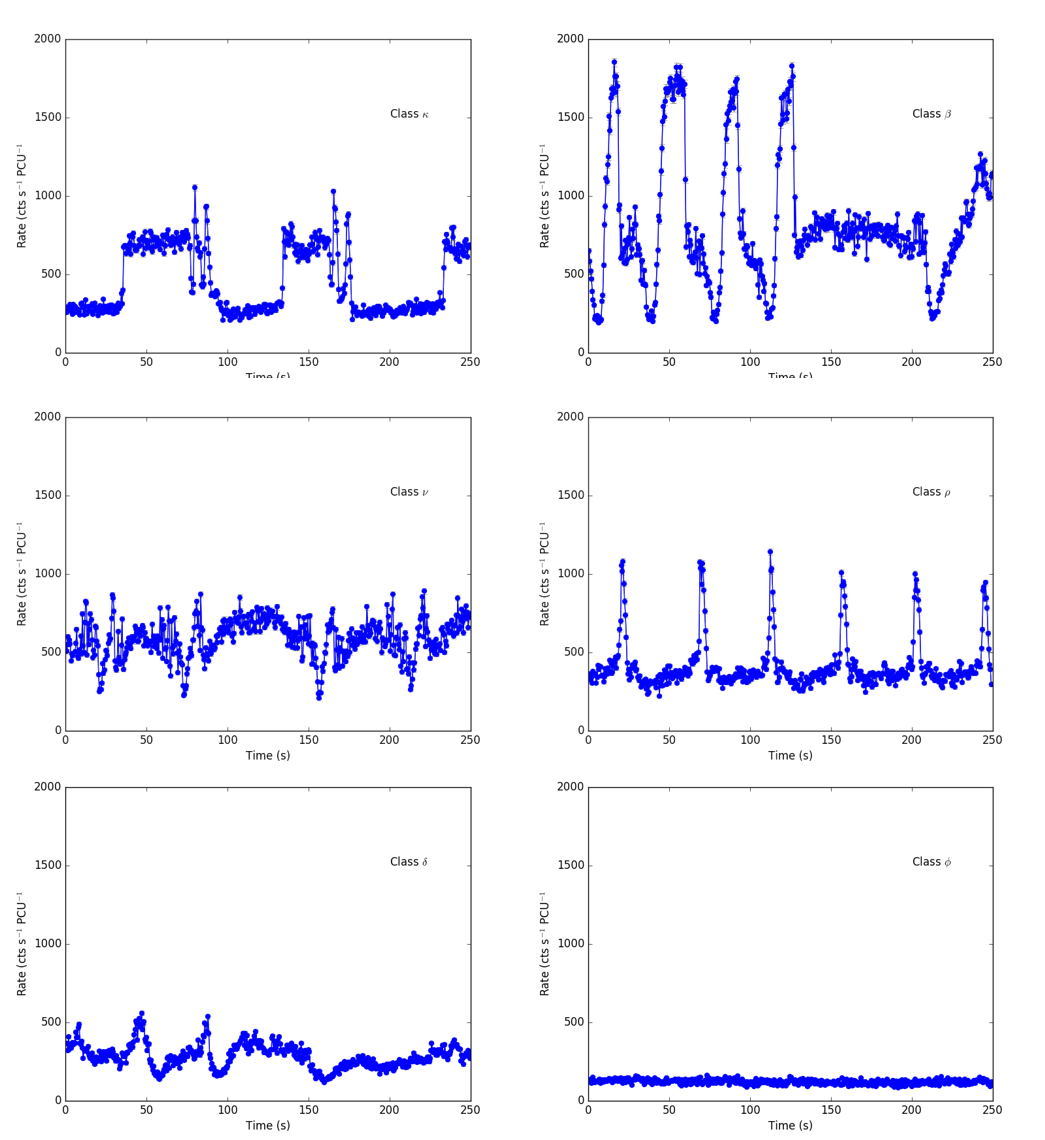
\includegraphics[width=\linewidth, trim= 0mm 0mm 5mm 0mm, clip]{images/GRSsample.png}
  \caption[Typical lightcurves of a selection of variability classes seen in the LMXB GRS 1915+105.]{Typical lightcurves of a selection of variability classes seen in GRS 1915, taken by the PCA instrument aboard \rxte .  The classes are labelled according to the Greek letter names assigned to them in \citet{Belloni_GRS_MI}.}
  \label{fig:GRSsample}
\end{figure}

\par The variability classes of GRS 1915 consist of a number of different types of variability, with a range of amplitudes and timescales.  Variability classes in GRS 1915 are usually denoted by the Greek letter names assigned to them by \citet{Belloni_GRS_MI}.  In general the variability associated with these classes takes the form of complex patterns of flares and dips, and it occurs over timescales of 10s to 100s of seconds.  In some classes, the variability is somewhat regular.  The $\rho$ class, also referred to as the `heartbeat' class due to the similarity of its lightcurve to the output of an electrocardiagram, consists of sharp quasiperiodic flares with a recurrence time of a few tens of seconds (Middle-right panel of Figure \ref{fig:GRSsample}).  Other classes, such as class $\kappa$ shown in the top-left panel of Figure \ref{fig:GRSsample}, consist of quasiperiodic fluctuations between two quasistable count rates: in the case of class $\kappa$, there is also a period of highly structured sub-second variability at each transition between these two classes.  Finally, two classes ($\chi$ and $\phi$, an example of the latter is shown in the bottom-right panel of Figure \ref{fig:GRSsample}) show no significant variability other than red noise; these classes are separated based on their spectral properties.  It has been suggested they they may be equivalent to the hard state seen in other outbursting LMXBs \citep{VanOers_GRSHard}, providing a possible link between the behaviour of GRS 1915 and the behaviour of more typical LMXBs.
\par The dramatic variability seen in GRS 1915 was long thought to be unique, driven by its unusually high accretion rate (e.g. \citealp{Belloni_Timescales}).  However in 2011, \citet{Altamirano_IGR_FH} identified GRS 1915-like variability in a second object: the black hole LMXB IGR J17091-3624 (hereafter IGR J17091).  This object is much fainter than GRS 1915: \citet{Altamirano_IGR_FH} showed that, assuming that this object accretes at its Eddington Limit by analogy with GRS 1915, the object may either be out in the halo of the Galaxy (at $\gtrsim20$\,kpc) or harbour the smallest mass black hole known to science ($\lesssim3$\,M$_\odot$).  The companion star to the black hole in this system has not been definitively identified \citep{Chaty_IGRCompanion}.
\par Much like GRS 1915, IGR J17091 displays a number of distinct classes of variability over time, and a number of these have been identified as being similar to the classes seen in GRS 1915 (e.g. \citealp{Altamirano_IGR_FH,Zhang_IGR}).  Unlike GRS 1915, IGR J17091 displays the pattern of outbursts and quiescence more commonly seen in LMXBs; known outbursts of IGR J17091 occurred in 2011 and 2016, and GRS 1915-like variability was observed in both \citep{Reynolds_2016HB}.
\par There are a number of notable differences between variability classes in GRS 1915 and IGR J17091.  In general, variability classes in IGR J17091 occur over shorter timescales than their counterparts in GRS 1915.  In addition to this, hard emission tends to lag soft emission in the variability classes of GRS 1915 (e.g. \citealp{Janiuk_Lag}), while the opposite trend has been found in the `heartbeat'-like class of IGR J17091 \citep{Altamirano_IGR_FH}.
\par In addition to GRS 1915 and IGR J17091, there have been claims that a third LMXB displays GRS 1915-like variability.  \citet{Bagnoli_RB} report on two observations of MXB 1730-335, also known as the `Rapid Burster', which show lightcurve patterns remarkably similar to those seen in the $\rho$ and $\theta$ classes of GRS 1915.  The presence of GRS 1915-like variability in the Rapid Burster is significant for a number of reasons: unlike GRS 1915 or IGR J17091, the Rapid Burster is known to contain a neutron star accreting at no more than 20\% of its Eddington Limit, thereby ruling out any black hole-specific or near-Eddington-specific explanations for this behaviour.  In addition to this, the Rapid Burster is one of only 2 objects known to undergo so-called Type II X-Ray bursts (see Section \ref{sec:TypeII}), suggesting a possible link between these two phenomena.  However, as it has only been observed twice in the $\sim30$ years since the object was discovered, the true nature of the apparent GRS 1915-like variability in the Rapid Burster remains unclear.

\subsection{A History of Models of GRS 1915-like Variability}

\par Over the years, a number of models and physical scenarios have been suggested to explain the complex variability seen in GRS 1915-like systems.  Successful models must also be able to explain why this type of variability is not seen in a wider array of sources.
\par One of the most best-studied classes of GRS 1915-like variability is Class $\rho$, the `heartbeat' class.  This variability class is present in both GRS 1915 and IGR J17091 (e.g. \citealp{Altamirano_IGR_FH}), and has been the focus of many of the models proposed to explain GRS 1915-like variability.  It has been shown that hard X-ray photons lag soft X-ray photons in this class (e.g. \citealp{Janiuk_Lag,Massaro_Lag}).  Other classes in GRS 1915 which show quasi-periodic flaring behaviour also exhibit this phase lag.
\par Previous authors have established models to explain both the hard photon lag as well as the `heartbeat'-like flaring itself, generally based on the instability in a radiation-dominated disk first reported by \citealp{Shakura_Instab} (see Section \ref{sec:diskinstab}).
\par \citealp{Belloni_Model1} first proposed an empirical model for flaring in GRS 1915.  They suggested that this behaviour is due to a rapid emptying of a portion of the inner accretion disk, followed by a slower refilling of this region over a viscous timescale.  These authors divided data from a given observation into equal-sized 2-Dimensional bins in count rate-colour space.  A spectral model was then fit to each of these bins independently to perform `pseudo'-phase-resolved spectroscopy (compare with the method outlined in Section \ref{sec:phasresspec}).  They showed that the quiescent time between flaring events correlates with the maximum inner disk radius during the flare; i.e., a correlation between the amount of the disk which is emptied and the time needed to refill it.  They go on to suggest that their model is able to explain all flaring-type events seen in GRS 1915.
\par The scenario proposed by \citealp{Belloni_Model1} was mathematically formalised by \citealp{Nayakshin_GRSModel}, who found that it was not consistent with a `slim' accretion disk \citep{Abramowicz_Slim} or with a disk in which viscosity $\alpha$ is constant with respect to radius.  As such, their model consists of a cold accretion disk with a modified viscosity law, a non-thermal electron corona and a transient jet of discrete plasma emissions which are ejected when the bolometric luminosity approaches the Eddington Limit.  Using this model, \citealp{Nayakshin_GRSModel} found that some formulations of $\alpha(r)$ result in the disk oscillating between two quasi-stable branches in viscosity-temperature space, over timescales consistent with those seen in the flaring of GRS 1915; they found that this occurs for accretion rates greater than 26\% of the Eddington limit.  They also found that by varying the functional form of $\alpha(r)$, their model gives rise to a number of lightcurve morphologies which generally match what is seen in data from GRS 1915.  \citealp{Janiuk_RadInstab} built on this model further by including the effect of the transient jet in cooling the disk; an effect not considered in the model by \citealp{Nayakshin_GRSModel}.  In this formulation, \citealp{Janiuk_RadInstab} found that GRS 1915-like variability should occur at luminosities as low as 16\% of Eddington.
\par \citealp{Belloni_GRS_MI} found that variability in GRS 1915 can be described by transitions between three phenomenological states, which differ in luminosity and hardness ratio.  This phenomenological scenario is at odds with the model of \citealp{Nayakshin_GRSModel}, which only results in two quasi-stable states.
\par \citealp{Nobili_Hotspot} tried to account for the hard X-Ray lag by supposing that a significant proportion of the X-Ray variability from the accretion disk comes from a single hotspot.  They suggest that the lag corresponds to a light travel time, after which a portion of this emission is Comptonised by the jet.  In this case, the geometric location of this hotspot determines the magnitude of this lag, and whether it is positive or negative.  This scenario goes some way to explaining why GRS 1915 is special, as it requires the presence of a jet during a soft-like state.
\par \citealp{Tagger_MagneticFlood} propose a magnetic explanation for the ejection of the inner accretion disk required by \citealp{Nayakshin_GRSModel} and \citealp{Janiuk_RadInstab}.  They suggest a limit cycle in which a poloidal magnetic field is advected towards the inner disk during the refilling of this region.  This field is then destroyed in reconnection events, releasing energy which results in the expulsion of matter from the inner disk.  They suggest that the three quasi-stable states proposed by \citealp{Belloni_GRS_MI} can be explained as states in the inner accretion disk with different values of plasma $\beta$.
\par \citealp{Janiuk_Lag} attempt to explain the hard lag in the heartbeats of GRS 1915 more simply, by proposing that it is caused by the non-thermal corona smoothly adjusting to changes in luminosity from the disk.  They base the variability of the disk on the model of \citealp{Nayakshin_GRSModel}, and show that the presence of a non-thermal corona which reacts to this variability naturally reproduces the lag behaviour seen in Class $\rho$ in GRS 1915.
\par \citealp{Merloni_MagDom} also propose a magnetic explanation for the reformulation of $\alpha(r)$ required by the model of \citealp{Nayakshin_GRSModel}.  Assuming that the viscosity in the accretion disk is dominated by turbulence due to magnetorotational instability, they find that allowing for a magnetically dominated corona naturally allows for the forms of $\alpha(r)$ required by \citealp{Nayakshin_GRSModel}.
\par \citealp{Zheng_Model} suggest that, when the effects of a magnetic field are included, the accretion rate threshold for GRS 1915-like variability should be $\sim50$\% of Eddington; significantly higher than the 16\% or 26\% reported by \citealp{Janiuk_RadInstab} or \citealp{Nayakshin_GRSModel}.  They go on to suggest that this sort of variability is only seen in GRS 1915 due to this source having the highest accretion rate of all permanently soft-state sources.  As such, this scenario still relies on a high accretion rate to trigger GRS 1915-like variability.%  However, magnetohydronamic simulations of a radiation dominated inner disk performed by \citealp{Hirose_Stable} suggest that the thermal instabilities required by models of heartbeat should not arise at any value of accretion rate.
\par \citealp{Xue_Spin} derive a mathematical model of the evolution of a slim accretion disk around a Kerr black hole.  They hypothesize that the spin of the black hole, not the accretion rate, may be the driving factor behind GRS 1915-variability.  However, they find that that the morphology of X-ray lightcurves from such a disk only has a weak dependence on the spin of the black hole, ruling this out as a possible explanation.
\par \citealp{Neilsen_GRSModel} performed phase-resolved spectroscopy of the $\rho$ class in GRS 1915.  They find a hard `spike' after each flare, which they associate with the hard lag in this class previously noted by e.g. \citealp{Janiuk_Lag}.  They propose a scenario in which high-velocity winds formed by the ejection of matter from the inner disk interact directly with the corona after a light travel time.  The corona then re-releases this energy as a hard bremsstrahlung pulse, causing the hard count rate spike seen in phase-resolved spectra.  This scenario is outlined in Figure \ref{fig:WindsModel}.  The authors expand this scenario in \citealp{Neilsen_Rho} to suggest that this mechanism can explain all classes in GRS 1915 which display $\rho$-like flaring.  However, this scenario still relies on the model of \citealp{Nayakshin_GRSModel} to generate the instability in the disk, and it implies that hard photons should always lag soft photons in heartbeat-like variability classes.

\pagebreak
\begin{figure}
  \centering
  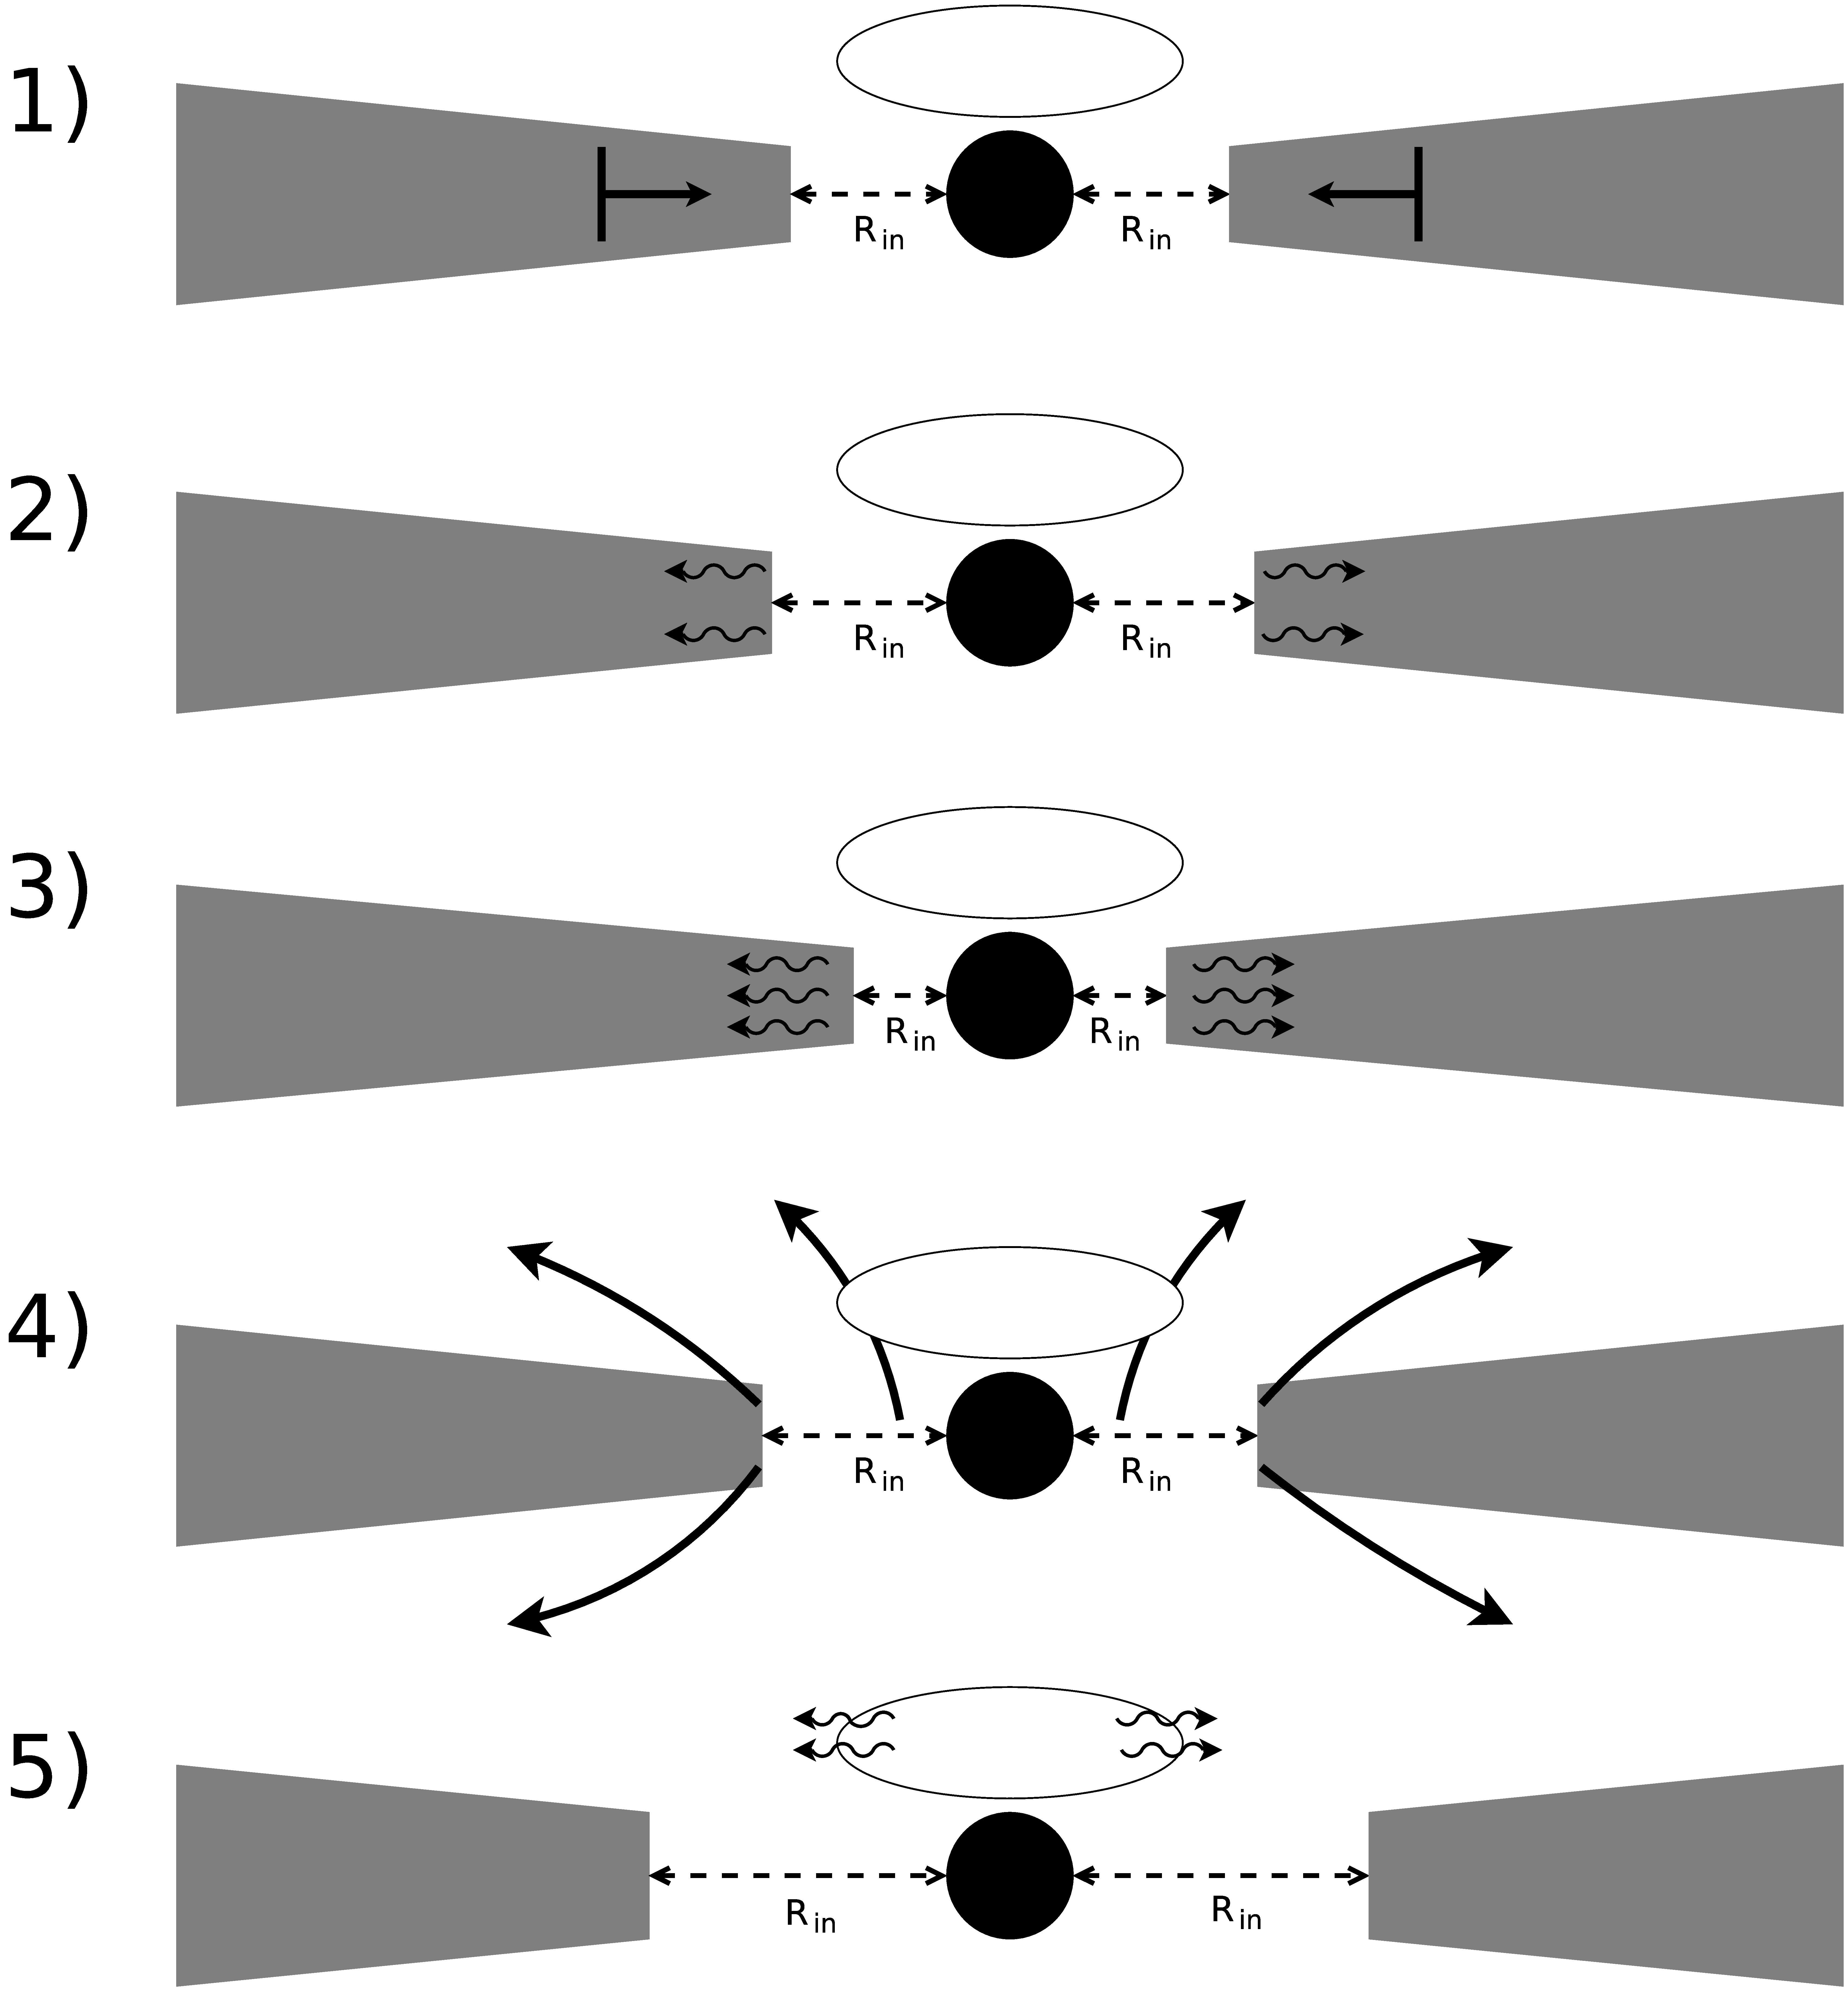
\includegraphics[width=.9\linewidth, trim= 25mm 0mm 0mm 0mm]{images/Wind_Model1.eps}
  \caption[A schematic diagram illustrating the the process described by \citet{Neilsen_GRSModel} to describe the $\rho$ variability class in GRS 1915+105.]{A schematic diagram illustrating the the process described by \citet{Neilsen_GRSModel} to describe the $\rho$ variability class in GRS 1915+105.  1) The X-ray emission from the system originates from both the accretion disc truncated at an inner radius $r_{in}$ (grey) and a cloud of non-thermal electrons (white ellipse).  At some time $t$, an overdensity in the accretion disc (formed by the instability described by \citet{Shakura_Instab}) propagates inwards towards $r_{in}$.  2) As the inner disc heats up, $r_{in}$ begins to slowly increase due to an increase in photon pressure.  This destabilises the disc.  3) At some critical density, the disc becomes too unstable and collapses inwards, greatly decreasing $r_{in}$ and raising the inner disc temperature.  4) The sudden increase in emission exceeds the local Eddington limit at $r_{in}$, ejecting matter from the inner accretion disc in the form of extreme winds.  5) Having been excited by matter in the winds passing through it, the non-thermal electron cloud emits a hard Brehmsstrahlung `pulse'.}
  \label{fig:WindsModel}
\end{figure}
\pagebreak

\par In their fitting, \citealp{Neilsen_GRSModel} consider three spectral models:
\begin{enumerate}
\item An absorbed disk black body with a high energy cutoff, of which some fraction has been Compton upscattered
\item An absorbed disk black body with a high energy cutoff, plus a Compton component with a seed photon spectrum tied to the emission from the disk
\item An absorbed disk black body plus a Compton component with a seed photon spectrum tied to the emission from the disk and a bremsstrahlung component
\end{enumerate}
They find that the first of these models (Model 1) is the best fit to the data.
\par \citealp{Mineo_PhasRes} also performed psuedo-phase-resolved spectroscopy of the $\rho$ class in GRS 1915, using a number of different spectral models to \citealp{Neilsen_GRSModel} but a significantly lower phase resolution.  In this work, the authors consider six models:
\begin{enumerate}
\item A multi-temperature disk black body plus a corona containing both thermal and non-thermal electrons (as forumlated by \citealp{Poutanen_Hybrid}).
\item A multi-temperature disk black body plus a multi-temperature disk black body plus a power law.
\item A multi-temperature disk black body plus an independent Compton component.
\item A multi-temperature disk black body plus a power law plus reflection from the outer disk.
\item A model of Comptonization due to the bulk-motion of matter in the disk.
\item A multi-temperature disk black body plus a power law plus a standard black body.
\end{enumerate}
With the exception of Models \textit{i} and \textit{vi}, the authors find that none of these models are able to satisfactorily fit the data in each of their phase bins independently.  As there is no reasonable physical explanation behind Model \textit{vi}, the authors only consider Model \textit{i}.  Their results suggest a large reduction of the corona luminosity during each heartbeat flare, which they interpret as the corona condensing onto the disk.  They also find that their results are consistent with GRS 1915 having a slim disk, but inconsistent with the hard lag being caused by photon upscattering in the corona.
\par \citealp{Massa_MoveLag} found that the magnitude of the lag between hard and soft photons in the $\rho$-class of GRS 1915 is not constant.  They found that the lag varies between $\sim3$--$10$\,s, and correlates strongly with count rate.  The magnitude of the lag, therefore, is too large to be simply due to a light travel time to the corona from the disk.  The authors suggest that their results are instead consistent the thermal adjustment of the inner disk itself as part of the instability limit cycle invoked to explain the flares.
\par \citealp{Massaro_Numerical} constructed a set of differential equations to mathematically explain the behaviour of the oscillator underlying $\rho$-like flaring in GRS 1915.  They find that a change between variability classes likely corresponds to a a change in global accretion rate, but that the accretion rate within the $\rho$ class is constant.  This model reproduces the count rate-lag correlation reported by \citealp{Massa_MoveLag}, as well as a previously reported correlation between flare recurrence time and count rate \citep{Massaro_Lag}.
\par \citealp{Mir_LagModel} instead propose a model of variability in the outer disk propagating inwards to the hotter inner disk.  They propose a model that explains both the hard lag of the fundamental frequency associated with the heartbeat flares, but also the hard lag of the first harmonic.  In contrast to the findings of \citealp{Massaro_Numerical}, their scenario requires a sinusoidal variation in the global accretion rate as a function of time.
\par More recently, \citealp{Zoghbi_Bulge} found that the reflection spectrum from GRS 1915 does not match what would be expected from the inner disk behaviour assumed by e.g. \citealp{Nayakshin_GRSModel}.  They again perform phase-resolved spectroscopy and fit a number of complex spectral models, finding that their data is best-described by the emergence of a bulge in the inner disk which propagates outwards during each flare.

\section{Type II Burst Sources}

\label{sec:TypeII}

\par Type II Bursts are another dramatic form of second-to-minute scale X-Ray variability which are thought to be caused by disk instabilities (e.g. \citealp{Lewin_TypeII}).  They are named by analogy to Type I X-Ray bursts; second-scale flashes of X-rays which are caused by thermonuclear explosions on the surface of neutron stars \citep{vanParadijs_TypeI,Lewin_Bursts}.
\par In general, Type II bursts can be defined as second-to-minute scale X-ray bursts from neutron star LMXBs which cannot be identified as Type I X-Ray bursts; specifically, they lack the power-law-like decay profile \citep{intZand_Decay} and spectral cooling \citep{Hoffman_T1Cool} seen in Type I bursts.  In Figure \ref{fig:BgB}, I show lightcurves of a number of Type II bursts from the LMXB MXB 1730-335 \citep{Bagnoli_PopStudy}.  Type II bursts have a fast rise and a slow decay, and occur with separation times from tens of seconds to hours.

\begin{figure}
  \centering
  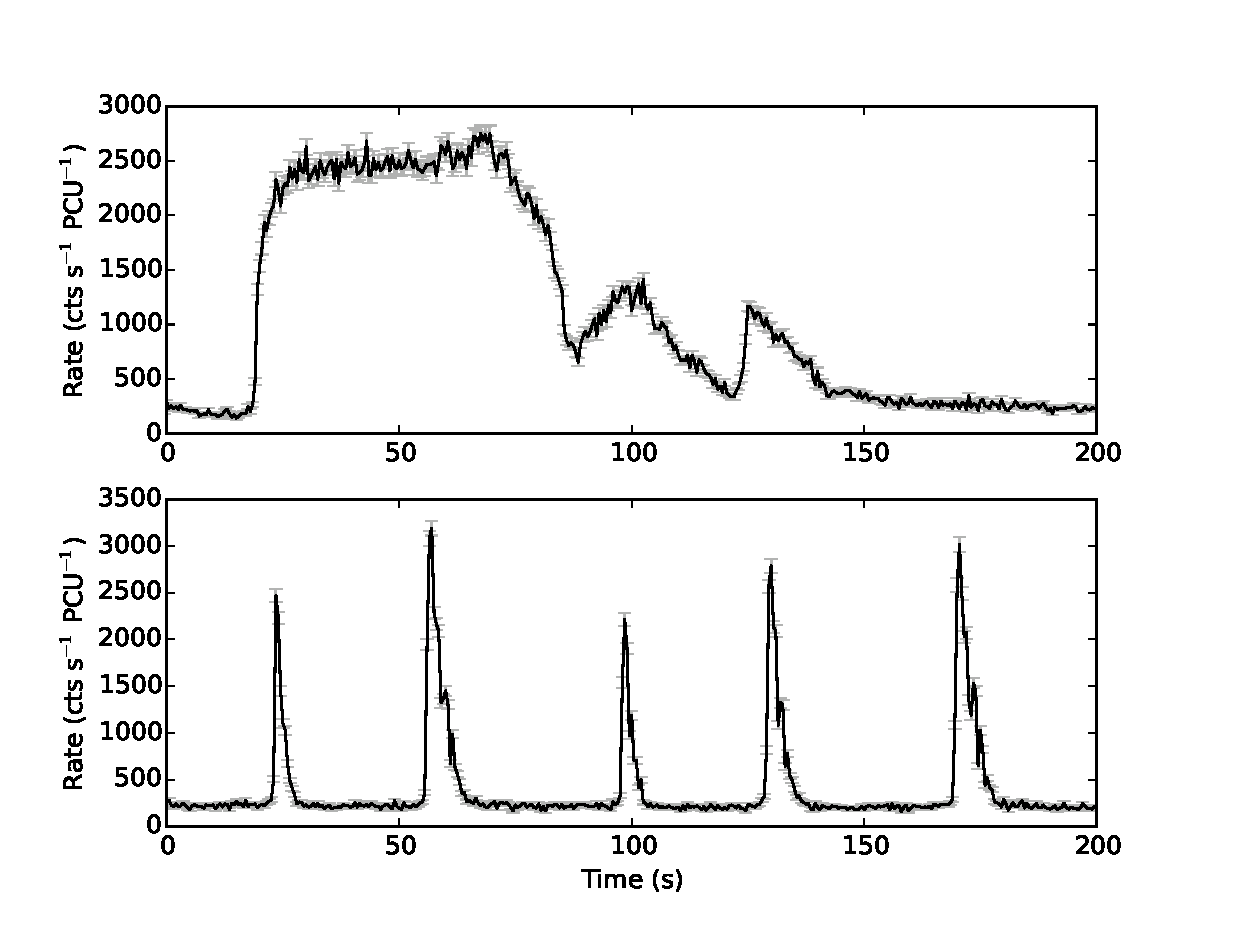
\includegraphics[width=.9\linewidth, trim= 0mm 0mm 0mm 80mm,clip]{images/bagnoli_bursts.eps}
  \caption[An \textit{RXTE}/PCA lightcurve of the Rapid Burster, showing a number of typical Type II X-ray bursts.]{An \textit{RXTE}/PCA lightcurve of MXB 1730-335 (also known at the `Rapid Burster', showing a number of typical Type II X-ray bursts.}
  \label{fig:BgB}
\end{figure}

\par Type II bursts have definitively been observed in only two objects: the neutron star LMXBs MXB 1730-335 (also known as the `Rapid Burster', \citealp{Lewin_TypeII}) and GRO J1744-28 (also known as the `Bursting Pulsar', \citealp{Paciesas_BPDiscovery}).  In both objects, Type II bursts have been observed during the soft state portion of multiple outbursts; this in turn suggests that the ability to produce Type II bursts is a property of the system, rather than the property of a specific outburst.  There have been claims of Type II-burst-like features during outbursts of a number of other LMXBs, such as SMC X-1 \citep{Angelini_SMC}, but whether these features are the same phenomenon remains unclear.
\par The Rapid Burster is an LMXB located in the globular cluster Liller 1 \citep{Lewin_TypeII}.  No pulsations have been detected from the system, and as such the spin of its compact object is not known.  However, the presence of Type I bursts from this object confirms that the compact object is a neutron star \citep{Hoffman_RB}.  Due to its location in a globular cluster, a number of infrared sources are consistent with the X-ray position of the Rapid Burster, and it is unclear which, if any, is the companion star in the system \citep{Homer_RBNoSec}.  However, also due to its association with Liller 1, the distance to the Rapid Burster is known to be 8.9--10\,kpc \citep{Ortolani_LillerD}.  Using this information, it has been shown that the persistent emission from the object during outburst peaks at no more than 20\% of its Eddington Limit \citep{Bagnoli_RB}.  The X-ray luminosity of the system at the peak of a Type II burst peaks at around 100\% of its Eddington Limit \citep{Tan_RBBursts,Bagnoli_PopStudy}.  In addition to Type I and Type II bursts, variability has been observed in the Rapid Burster which is remarkably similar to that associated with GRS 1915 and IGR J17091 (see Section \ref{sec:1915}), suggesting a possible link between these types of variability.
\par The Bursting Pulsar is an LMXB located in a region of the sky very close to the Galactic centre.  Although Type I bursts have not been observed from this system, a coherent 2.14\,Hz X-ray pulsation seen from the object proves that the compact object is a pulsar \citep{Kouveliotou_BPPulse}.  The distance to the object is $\sim3.4$--4.1\,kpc \citep{Sanna_BP}, and the nature of the companion star is unknown.  The persistent emission from the Bursting Pulsar is believed to peak at $\sim100$\% of its Eddington limit during outbursts, while its peak luminosity during Type II bursts greatly exceeds the Eddington limit \citep{Sturner_BPNature}.

\subsection{A History of Models of Type II Bursts}

\label{sec:TIImod}

\par No models have been proposed which can fully explain Type II bursting behaviour, but several models have been proposed in the context of Type II bursting from the Rapid Burster MXB 1730-33.  A number of models invoke viscous instabilities in the inner disk as the source of cyclical bursting.  One such example was presented by \citet{Taam_Evo} xxxxx
\par \citet{Hayakawa_Type2Mod} xxxxx but these fail to explain why the majority of Neutron Star LMXBs do not show this behaviour.
\par \citet{Walker_Type2Mod} suggests that, for a neutron star with a radius less than its ISCO, a similar cycle of accretion can be set up when considering the effects of a high radiative torque.  All of these models suggest that Type II bursts are caused by sporadic accretion events onto the neutron star, which in turn are caused by instabilities that originate in the inner part of the accretion disk.  For a more detailed review of these models, see \citet{Lewin_Bursts}. xxxxx
\par \citet{Spruit_Type2Mod} use a different approach.  They show that, in some circumstances, the interaction between an accretion disk and a rapidly rotating magnetospheric boundary can naturally set up a cycle of discrete accretion events rather than a continuous flow  (see also \citealp{Dangelo_Episodic1,Dangelo_Episodic2,vandenEijnden_RB,Scaringi_Gating}). xxxxx